\chapter{Estudo para aplicação do projeto em Realidade Aumentada}

Este trabalho de projeto de formatura teve parte de seu desenvolvimento realizado na disciplina de Interface Humano Computador. Na ocasião, foi necessário realizar um projeto de estudo de usuário como parte da avaliação na disciplina e com isto surgiu-se a possibilidade de se implementar uma solução em Realidade Aumentada (RA) como parte do projeto.\\

Uma pesquisa de estudo de usuário se justifica por buscar a melhor experiência para os biólogos primatologistas, os quais são os usuários finais deste sistema. No que se refere a uma implementação em RA, a ideia abrange a atuação do pesquisador em campo e a sua implementação o auxiliaria então a localizar os animais monitorados. O dispositivo utilizado deve ser capaz de mostrar uma projeção do ambiente com sinalização da localização dos animais e detalhes de interesse.

Neste apêndice, são apresentados os resultados obtidos da pesquisa realizada para uma possível implementação em Realidade Aumentada do projeto SIMIOS. Ela incluiu uma serie de perguntas feitas a um conjunto de entrevistados, bem como a elaboração de um termo de consentimento feito na época para acordo destes entrevistados.

\section{Stakeholders}

São usuários primários veterinários e pesquisadores que realizam trabalho de campo em reservas naturais, que usarão o sistema com frequência. Usuários secundários são estudantes de biologia ou veterinária que ocasionalmente realizem trabalho de campo acadêmico. Demais usuários poderiam ser visitantes de parques naturais interessados em ver animais silvestres.

\section{Papéis e Variáveis de Perfil}

Foram identificados os seguintes papéis:

\begin{enumerate}
\item Veterinário - trabalha diretamente com o animal e se preocupa essencialmente com o bem estar e saúde do mesmo (mais preocupado com informações que reflitam sua condição corporal);
\item Pesquisador (biólogo/psicólogo/estudante) - trabalha distanciado do animal, se preocupando em obter informações relacionadas ao comportamento do mesmo;
\item Visitantes (turistas) - interessados em localizar e interagir o máximo possível com os animais.
\end{enumerate}

O pesquisador é escolhido como usuário primário para ser alvo do estudo. Para este papel, as variáveis relevantes levantadas são:

\begin{itemize}
\item Formação acadêmica (curso e grau): identifica a profundidade da pesquisa que é realizada
\item Qual reserva o pesquisador trabalha: dimensiona o tamanho e a quantidade de animais que são monitorados;
\item Há quanto tempo a pessoa trabalha com esse tipo de pesquisa: identifica o grau de experiência do usuário;
\item Quanto tempo do seu ofício é dedicado ao monitoramento dos macacos: identifica a ênfase que é dada à tarefa.
\end{itemize}

\section{Necessidades}

As perguntas elaboradas que expressam a motivação deste trabalho são:

\begin{enumerate}
\item Quais são alguns dos procedimentos padrão do pesquisador/veterinário de campo? O que é feito e onde?
\item Como é feito para localizar um macaco específico?
\item Que tipos de equipamentos e ferramentas são manipulados?
\item Quais informações são necessárias?
\item Que tipo de planejamento prévio é realizado para executar bem essa atividade?
\item A forma como tudo isso é feito te agrada? Existem dificuldades?
\end{enumerate}

\section{Instrumentos}

A primeira técnica selecionada foi o questionário, pois, apesar de conter perguntas mais fechadas, é mais abrangente, podendo atingir vários perfis. A segunda sendo a entrevista que, por outro lado, pode engatilhar discussões mais abertas com o entrevistado ao mesmo tempo que não atingirá muitos stakeholders (planeja-se entrevistar preferencialmente usuários primários).
Pelo fato de os usuários primários constarem de um grupo bem fechado cuja disponibilidade é limitada, optou-se pela entrevista por dois motivos essencialmente. Primeiro, por ser uma técnica que exigirá uma quantidade menor de entrevistados e, segundo, por encaixar mais no perfil de dinâmica privativa e rápida que se pode esperar que os pesquisadores corroboram em participar.
Ambas as técnicas selecionadas são reflexivas (que exercitam a reflexão do usuário sobre o sistema, não avaliando seu comportamento à exposição do mesmo). A entrevista, no entanto, é qualitativa, ao passo que o questionário tenta quantificar a opinião dos usuários.
Foi feito um formulário do Google para ser distribuído como questionário e utilizado como auxílio ao entrevistador. A entrevista foi dada por uma conversa gravada com duração de 1 hora com a profª drª Cristiane Pizzutto da FMVZ (USP).

\section{Amostra}

O questionário pode envolver quantas pessoas conseguir atingir, considerando que potencialmente alguma parte delas esteja fora dos papéis levantados - que, então, ou serão desclassificadas ou acrescentarão para a composição de papéis.
A entrevista, por focar mais em um grupo bem específico de usuários e de relativo difícil acesso, espera-se que será possível contar com a participação de entre um ou dois usuários.

\section{Resultados}

As respostas obtidas através do questionário podem ser observadas no Anexo A deste documento. O questionário provavelmente sofreu determinado viés pelo fato de ter sido distribuído em meios sociais em que a maioria massiva do público presente era de jovens universitários brasileiros. Isso é comprovado, como pode ser observado, pela faixa etária (entre 19 e 26 anos) e pela formação acadêmica (graduação) obtidas.
Ademais, foi possível concluir que não é tão simples encontrar universitários com qualquer experiência prática em pesquisa com animais. Ainda assim, os mesmos participantes inexperientes se mostraram interessados pelo projeto sendo desenvolvido. Dessa forma, pode-se concluir que seria importante que o dispositivo tivesse um direcionamento para ser mais educativo, focado no treinamento de novos pesquisadores.
Assim, o primeiro perfil levantado é o seguinte:

\begin{table}[ht]
\centering
\caption{Primeiro Perfil Levantado}
\vspace{0.5cm}
\begin{tabular}{| l | l | m{8cm} |}
\hline
\multirow{5}{*}{
\includegraphics[scale=0.35]{table6-primeiroperfil}} & Identidade & Cristian La Roche, 23 anos\\ \cline{2-3}
& Status & Pesquisador\\% \vspace{0.4cm}\\ %\vspace{0.4cm}\\ \cline{2-3} 
& Formação Acadêmica & Estudante recém graduado em medicina veterinária\\ %\vspace{0.4cm} \\ \cline{2-3}
& Experiência em Campo & Nunca fez pesquisa de campo envolvendo animais\\ %\vspace{0.4cm} \\ \cline{2-3}
& Expectativas & Acredita que ter auxílio de realidade aumentada pode ajudá-lo na atividade\\ %\vspace{0.4cm}\\ 
\hline
\end{tabular}
\vspace{0.4cm}\\
\centerline{\small{Fonte: autores}}
\end{table}

\FloatBarrier

Da entrevista, foi possível tirar duas conclusões principais. A primeira é que para os pesquisadores o mais relevante é conhecer informações relacionadas aos sinais vitais do animal - tais como a frequência cardíaca, a temperatura corporal e a movimentação - em tempo real. Segundo, é possível perceber que pesquisadores que trabalhem em cativeiro são, também, possíveis usuários do sistema, desde que o mesmo seja capaz de transmitir tais informações.
Além disso, foram apontadas como dificuldades que potencialmente sanadas pelo sistema o registro e exibição dos dados coletados e a identificação individual de alguns animais silvestres, como cangurus.
A entrevistada relatou ter tido problemas em se acostumar com software auxiliar no passado, mas culpa a baixa usabilidade do mesmo. Apesar disso, se mostrou bastante interessada em integrar qualquer meio tecnológico que se apresentasse capaz de auxiliar a pesquisa.
Assim, foi possível criar um segundo perfil:

\begin{table}[ht]
\centering
\caption{Segundo Perfil Levantado}
\vspace{0.5cm}
\begin{tabular}{| l | l | m{8cm} |}
\hline
\multirow{5}{*}{
\includegraphics[scale=0.35]{table7-segundoperfil}} & Identidade & Brenda Araújo, 36 anos\\ \cline{2-3}
& Status & Pesquisadora\\% \vspace{0.4cm}\\ %\vspace{0.4cm}\\ \cline{2-3} 
& Formação Acadêmica & Doutorado em Medicina Veterinária\\ %\vspace{0.4cm} \\ \cline{2-3}
& Experiência em Campo & Frequentemente visita cativeiros de animais silvestres a trabalho.\\ %\vspace{0.4cm} \\ \cline{2-3}
& Expectativas & Não tem muita facilidade com novas tecnologias mas aceita o desafio em prol dos animais.\\ %\vspace{0.4cm}\\ 
\hline
\end{tabular}
\vspace{0.4cm}\\
\centerline{\small{Fonte: autores}}
\end{table}

\FloatBarrier

\section{Registro das respostas do questionário}

Inicialmente, foram feitas perguntas relacionadas às variáveis apontadas no item 3. Nem todas as variáveis foram incluídas pois algumas delas se fizeram claras somente após discutidos os resultados do questionário.

\begin{figure}[ht]
  \centering
    \caption{Quantos anos você tem?}
    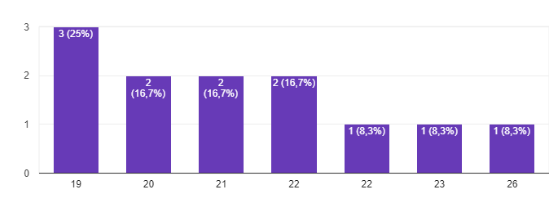
\includegraphics[scale=0.6]{anexo7-quantosAnosVoceTem}
	\centerline{\small{Fonte: autores}}
\end{figure}
\FloatBarrier

\begin{figure}[ht]
  \centering
    \caption{Qual sua área de atuação?}
    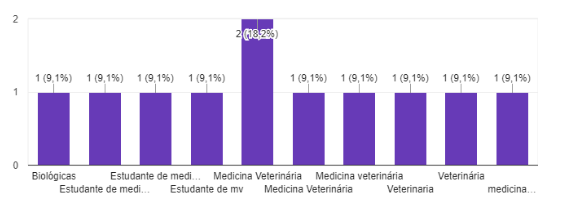
\includegraphics[scale=0.6]{apendice7-qualSuaAreaDeAtuacao}
	\centerline{\small{Fonte: autores}}
\end{figure}
\FloatBarrier

\begin{figure}[ht]
  \centering
    \caption{Qual sua formação?}
    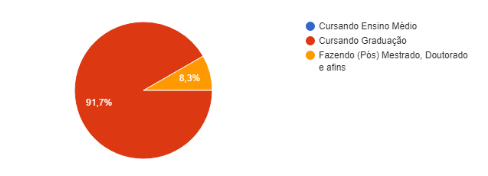
\includegraphics[scale=0.65]{apendice7-qualSuaFormacao}
	\centerline{\small{Fonte: autores}}
\end{figure}
\FloatBarrier

\begin{figure}[ht]
  \centering
    \caption{Já participou de pesquisa de campo envolvendo animais?}
    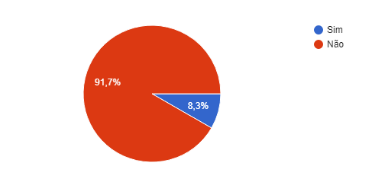
\includegraphics[scale=0.65]{apendice7-pesquisaAnimais}
	\centerline{\small{Fonte: autores}}
\end{figure}
\FloatBarrier

\begin{figure}[ht]
  \centering
    \caption{Já participou de pesquisa em laboratório envolvendo monitoramento do comportamento de animais?}
    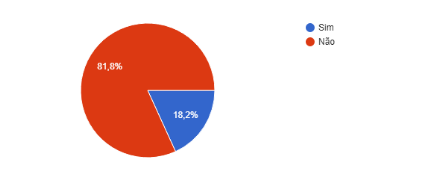
\includegraphics[scale=0.65]{apendice7-pesquisaLaboratorio}
	\centerline{\small{Fonte: autores}}
\end{figure}
\FloatBarrier

\section{Mapa do Desafio}

Após feito o estudo do Usuário, chegou-se numa ideia de prototipação de como a solução em Realidade Aumentada poderia ser. \\

O mapa de desafio visa mostrar a sequência de ações tomadas pelos usuários da interface de RA durante a utilização do sistema SIMIOS.


\begin{sidewaysfigure}[ht]
  \centering
    \caption{Mapa do Desafio}
    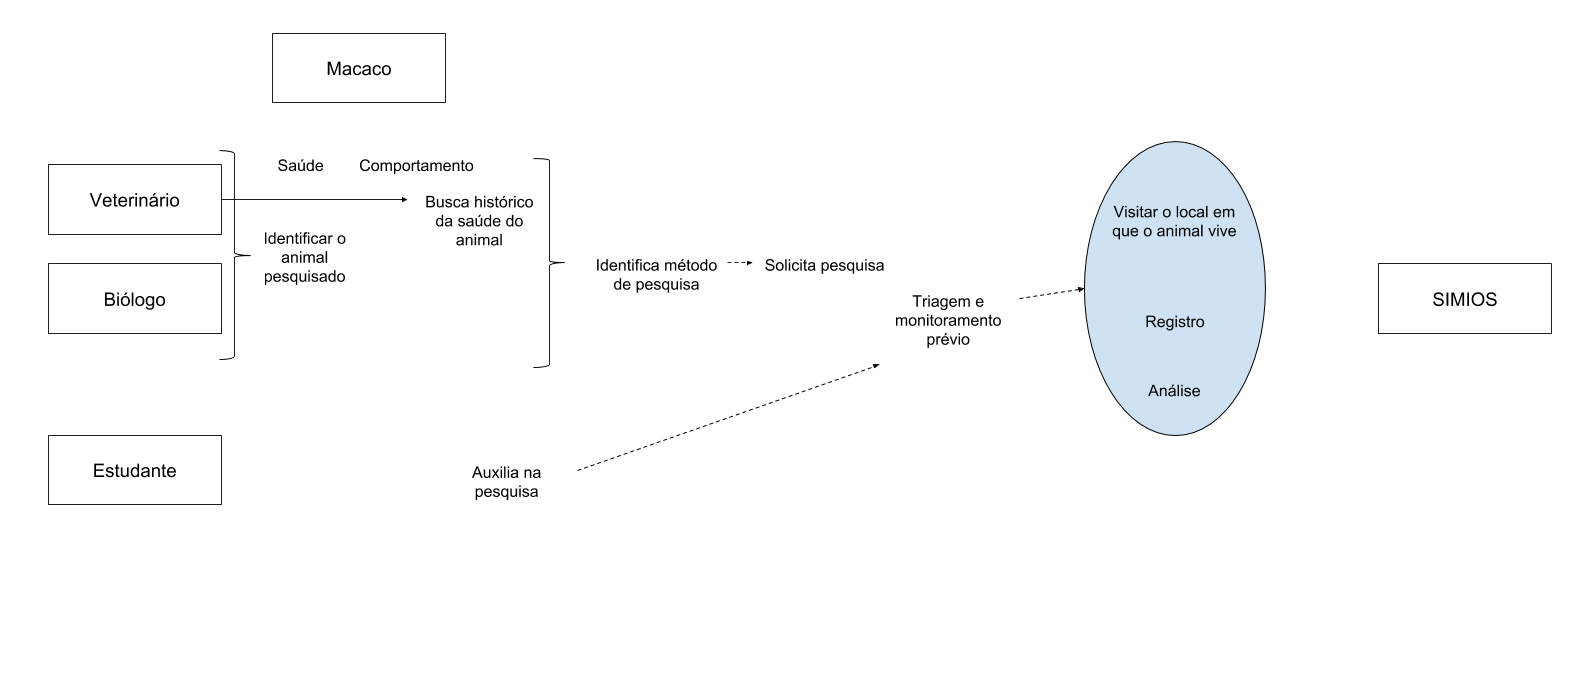
\includegraphics[scale=0.40]{anexo7-mapadodesafio}
	\centerline{\small{Fonte: autores}}
\end{sidewaysfigure}
\FloatBarrier